\documentclass{article}
\usepackage[utf8]{inputenc}
\usepackage{subfig}
\usepackage{amsmath}

\usepackage{graphicx}
\usepackage[legalpaper, portrait, margin=0.5cm]{geometry}

\thispagestyle{empty}

\begin{document}

\begin{figure}[h]
        \centering
        \subfloat[$\epsilon_{e}\gg\epsilon_{u}$]{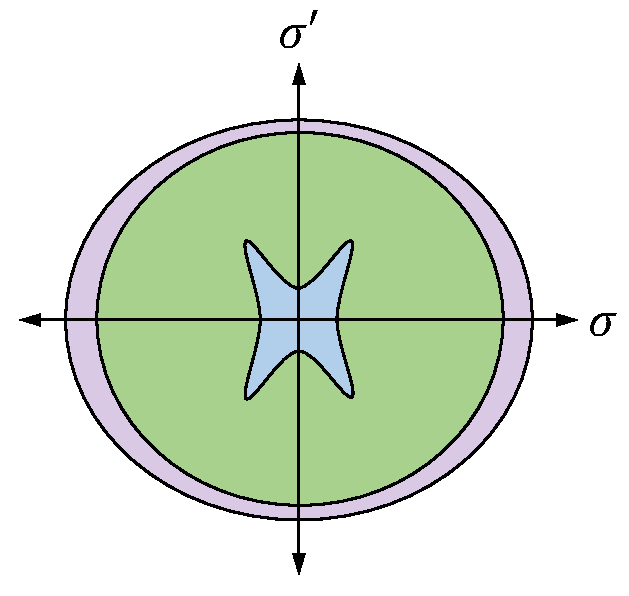
\includegraphics[height=3.1cm]{figures/ch02/e_larger_u.pdf}}
        \subfloat[$\epsilon_{e}\sim\epsilon_{u}$]{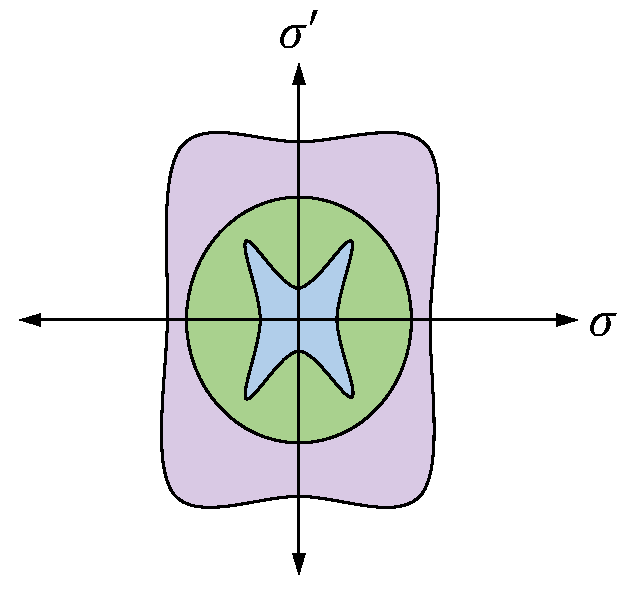
\includegraphics[height=3.1cm]{figures/ch02/e_equal_u.pdf}}
        \subfloat[$\epsilon_{e}\ll\epsilon_{u}$]{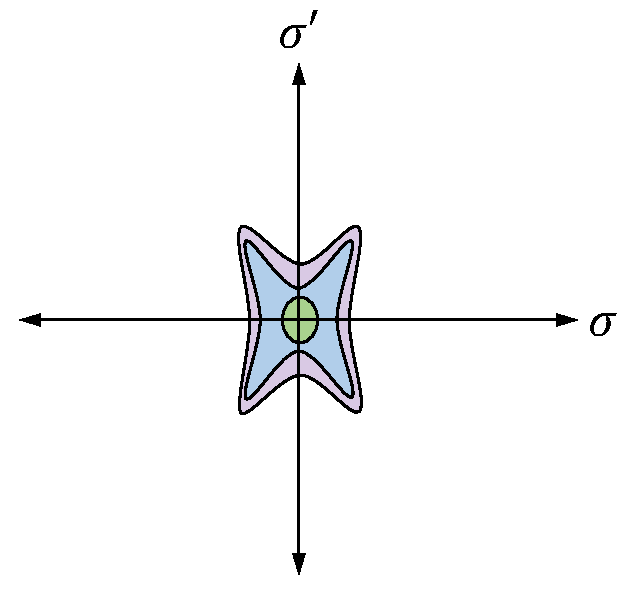
\includegraphics[height=3.1cm]{figures/ch02/e_smaller_u.pdf}}\\
        \includegraphics[width=4cm]{figures/ch02/02_e_u_legend.pdf}\\



        
\end{figure}


\end{document}